\section{London --- London Congestion Charge}

\subsection{History}

Beginning in the 1960's, downtown pricing in London was the focus of constant study. \citet{Thomson1967a} considered a \pounds XXX daily license using stickers required for travel between 8AM and 7PM in an area of central London north of the Thames. In the 1970's, the Greater London Council---a governing body over London's many small boroughs founded in 1968---commissioned research on a supplementary license for a larger zone that included all the land inside the London Inner Ring Road (including land south of the Thames) \citep{may1975}, which is the area London wound up using for the London Congestion Charge in 2003. But though research predicted large benefits, the Greater London Council rejected the particular scheme design, citing concerns with equity and enforcement \citep{Richards2006}. In 1986, due to the antogonism of the Council's leftist leader, Ken Livingston, the Conservative national government replace the Greater London Council with a less powerful body called the London Planning Advisory Committee (LPAC). LPAC endorsed  then comissioned several very detailed and advanced studies on different scheme designs, which are described in \citet[p. 51-54]{Gomez-Ibanez1994}. Afterward, from 1991 to 1994, the UK Department of Transport launched the London Congestion Charging Research Programme, a series of still more detailed studies \citep{MVA1995,Richards1996}, but at their conclusion the Secretary of State for Transport decided that the technological problems loomed too large for the time being.

Concrete steps toward road pricing in London finally began in the late 1990's. In May 1997, the UK elected a new Labour government, who shortly called a referendum on the question of creating a Greater London Authority---a regional government similar to the Greater London Council abolished in 1986---which would be headed by a Mayor of London. In May 1998, this proposal won the referendum by a large margin. Since Labour policy papers suggested the new Mayor's powers would include enacting downtown pricing, in August 1998 the Government Office for London convened a team of experts, the Road Charging Options for London (ROCOL) Working Group, to study the matter one last time. In 1999, Parliament passed the Greater London Authority Act \citep{Parliament1999}, which did give the Mayor such powers; and in March 2000 ROCOL published its final report, \citep{ROCOL2000}.

Ken Livingstone---who had included downtown pricing in his election manifesto---won the first mayoral election in May 2000. After being briefed on \citet{ROCOL2000}, Livingston decided to move forward with enforcement by Automatic Number Plate Recognition (ANPR) cameras. ROCOL had also considered paper licenses and transponder systems, but cautioned that the former were impractical and the latter would mean delaying the scheme beyond the Mayor's first term: national authorities were still working on national standards for transponder charging. After two years of preparation and consultation with the public, the London Congestion Charge went into effect on February 17th, 2003.

\subsection{Design}

The LCC launched as a \pounds5 charge for travel between 7:00 AM and 6:30 PM within the 22 km$^{2}$ Charging Zone (CZ). The CZ is the solid region in Figure \ref{fig:London-Congestion-Charging} and is the same zone considered by \citet{Thomson1967a}. Uniquely, the LCC covers all travel within the zone---not just traversals of a cordon like the other schemes---as well as vehicles that are merely parked on the street. Therefore, enforcement requires ANPR cameras (over 500 at the launch) mounted on poles throughout the zone and along its boundaries, as well as cameras mounted on patrolling vans. Paying once buys unlimited same-day usage. The baseline payment method is as follows: if one uses public streets in the CZ during charging hours, one has until midnight to pay by calling a number, SMS, a website, payment machines or in various stores. Non-payment results in a penalty being issued to the vehicle's registered owner.

The LCC has undergone a number of minor changes of which we will list only a few. The toll was raised from \pounds5 to \pounds8 in July 2005, \pounds10 in January 2011 and \pounds11.50 in June 2014. In 2007, the end of charging was moved up from 6:30 to 6:00 PM. Since June 2006, if one pays by midnight on the day after visiting the zone the penalty is small (\pounds 2.50). Since January 2011, an Auto Pay option has let customers pay automatically and earn a \pounds 1 discount.

There are myriad exemptions and discounts.\footnote{See \citet[Table 1, p. 515]{Santos2005} for a tabulated list that is almost unchanged today.} Using Auto Pay earns a \pounds1 discount. Residents receive a 90\% discount. Motorcycles, buses, vehicles with 9+ seats, licensed taxis/mini-cabs, certain emergency and vehicles, certain vehicles used for or by  disabled people, and certain vehicles with very low emissions are all completely exempt or eligible for a ``100\% discount,'' which, unlike exemption, requires registration and possibly a small fee.

In February 2007, TfL added a 19 km$^{2}$ area called the ``Western Extension'' (the striped area in Figure \ref{fig:London-Congestion-Charging}). But after a consultation showed the public heavily opposed \citep{TfL2008b}, it was abolished in January 2011.

\begin{figure}[ht]
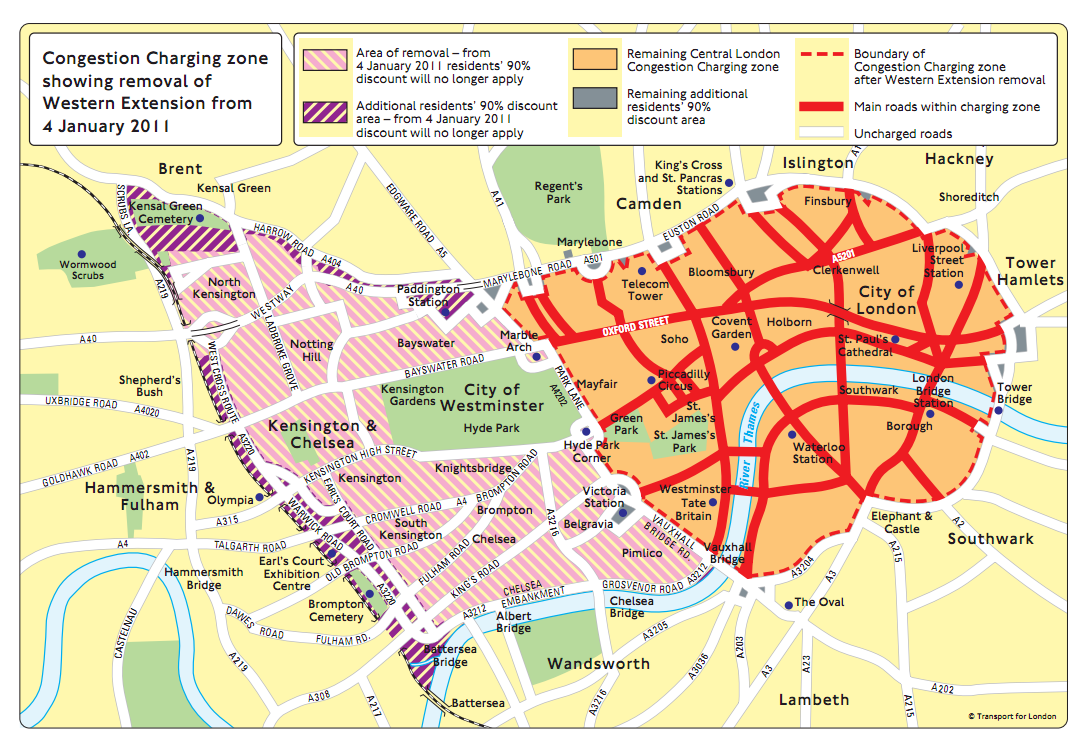
\includegraphics[width=0.95\linewidth]{../img/london-congestion-charge.png}

\caption{London Congestion Charging Zone (Transport for London, 2015)\label{fig:London-Congestion-Charging}}
\end{figure}

\subsection{Results}

In the first year of operation, entries by private car during charging hours fell 33\% (65,000 per day) and entries by all chargeable vehicles fell 27\% (73,000 per day). By contrast, entries by private taxi, which were exempt from charging, jumped 18\% (10,000). These patterns held steady over the years 2003-2007 when TfL published its monitoring reports. There was little sign of a switch to subway (metro), but bus ridership grew rapidly \citep[p. 58]{TfLFifth2007}, partly due to the Charge itself and partly due to service improvements wrought by the revenue the Charge raised. 

In the first year, the LCC produced a mild fall in travel times, but by 2007 the original  drop had dissipated. TfL has blamed long-term deterioration in the capacity of the road network, because similar falls in speed---adjusted for flows---was observed outside the charging zone and at night (see \citet[p. 45-55]{TfLFifth2007} and CITE TRAVEL IN LONDON REPORT 2, Sec 11.10). The agency has suggested this fall in capacity could be attributed to construction and to projects such as bus lanes, bus priority and pedestrian or cycling safety measures. Thus, in some sense, the LCC can be looked at not as a way to \emph{raise} traffic speeds but rather as a way to \emph{maintain} traffic speeds while obtaining other public goods and permitting substantial construction.  TfL itself suggests as much: ``The loss of highway capacity accelerated, in central London particularly,
after the introduction of congestion charging. This may have been due to highway authorities taking advantage of the reduced traffic demand for road space, following the introduction of charging, to reallocate capacity to other beneficial uses'' (CITE TFL TRAVEL IN LDON REPORT 4 p. 103).

\begin{figure}[ht]
    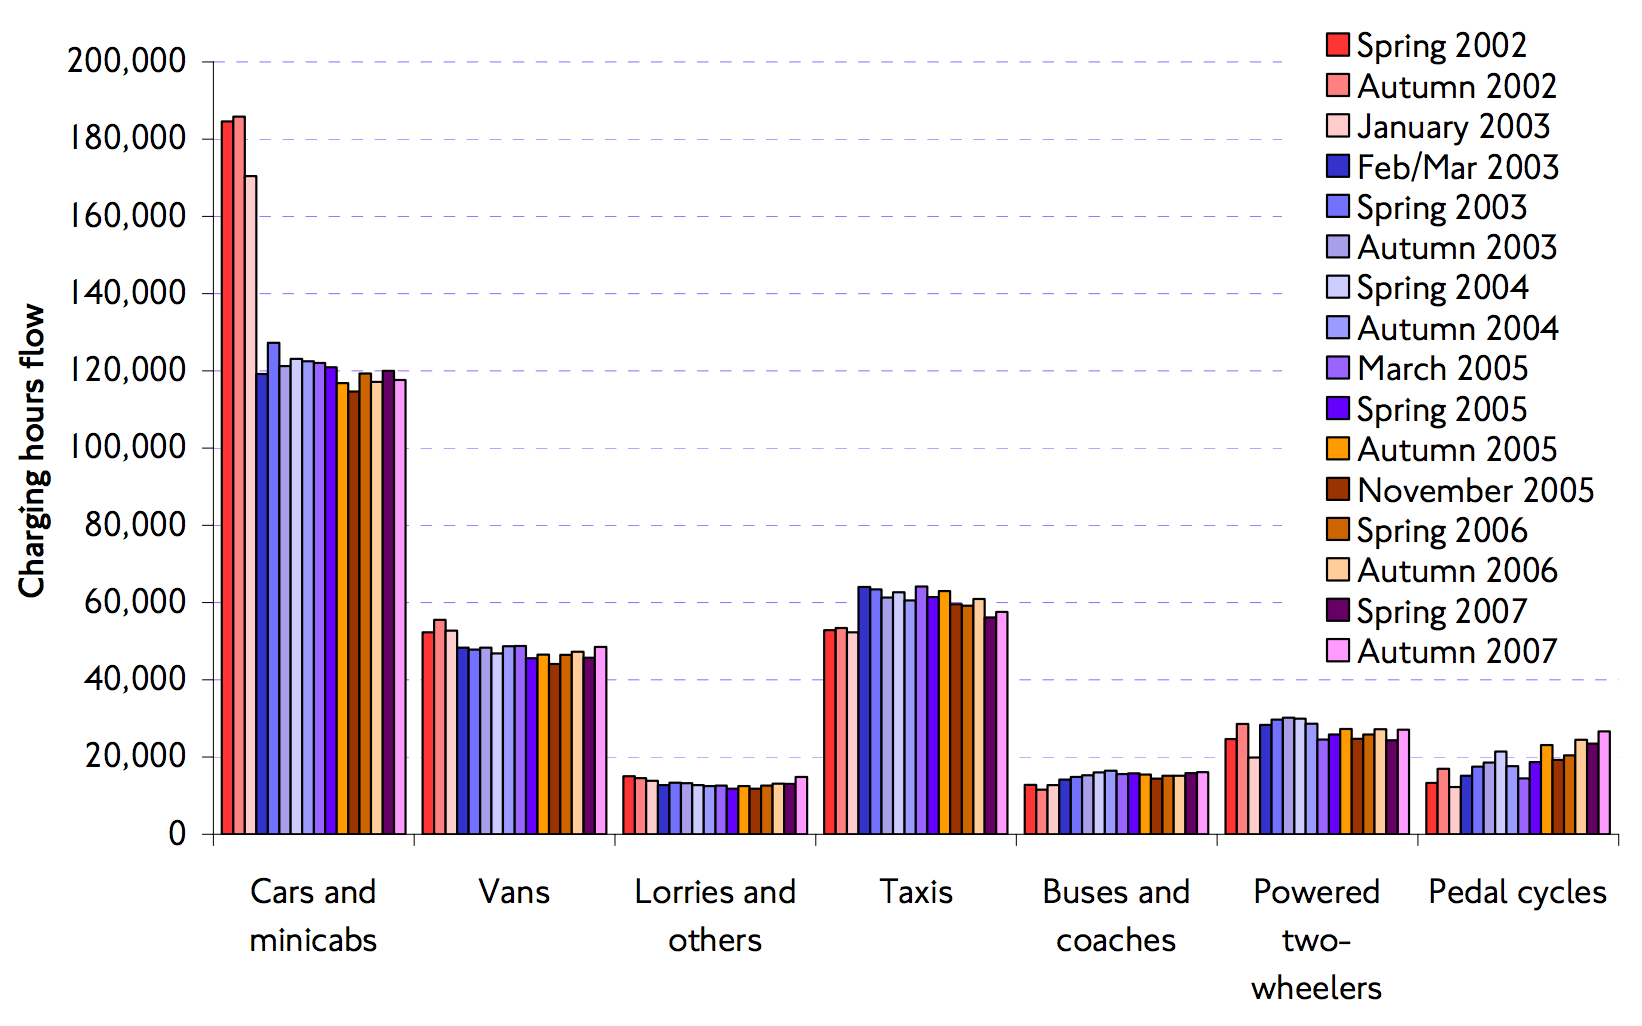
\includegraphics[width=.95\textwidth]{../img/london-entries.png}
    \caption{Entries to the original LCC charging zone by traffic type. \citep[p. 20]{TfLFifth2007} } \label{fig:london-entries}
\end{figure}

% \begin{figure}[ht]
%     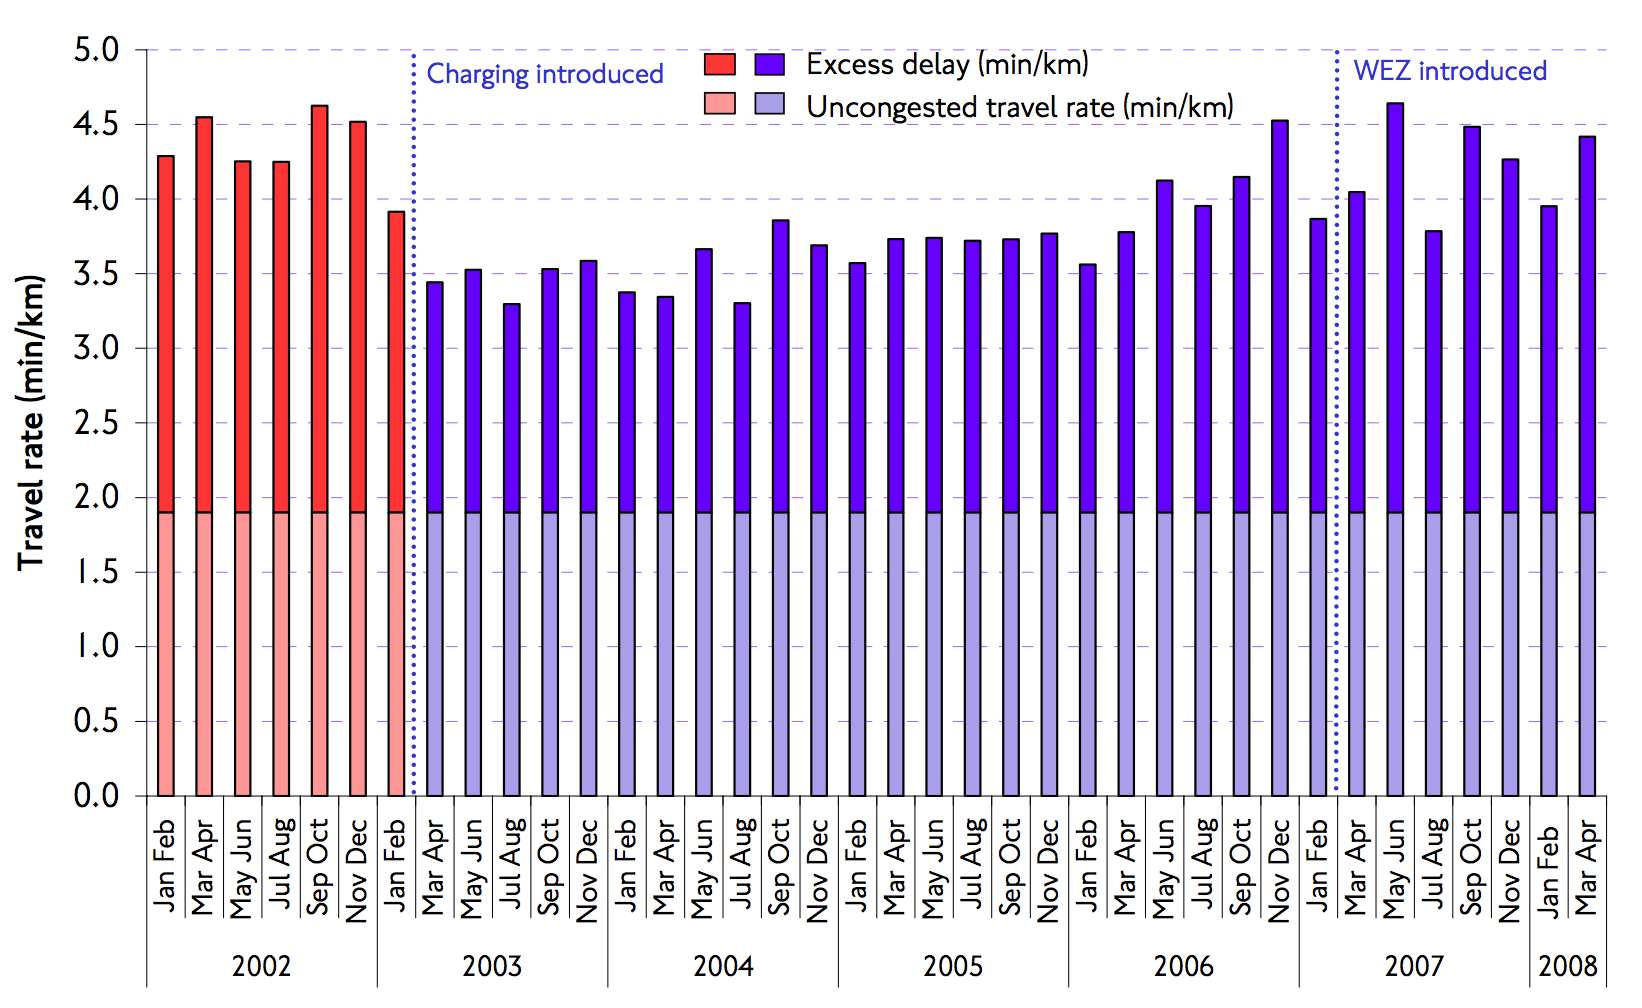
\includegraphics[width=.95\textwidth]{../img/london-travel-times.png}
%     \caption{Entries to the original LCC charging zone by traffic type. \citep[p. 20]{TfLFifth2007} } \label{fig:london-travel-times}
% \end{figure}



% Talk about speed disappointment.

\subsection{Finances}

Financially, the LCC failed to live up to expectations. \citet{ROCOL2000} predicted setup costs would be about \pounds30-50 million, annual operating costs in the same range and \pounds230-270 million in annual revenue (CITE PAGE NUMBER). See Table \ref{tab:London-Congestion-Charge}. A chief reason for the shortfall was that car entries fell more (30\%) than expected (20\%) (CITE DIFFERENT \citep[p.169]{Leape2006}). \citet{TfLExPost2007} reports that only 40 percent of daily entries pay the full charge. Note that penalties (for the years when such data are available) accounted for substantial revenue. Years 2008-2011 in Table \ref{tab:London-Congestion-Charge} are starred to highlight the years of the Western Extension---a time of higher costs and revenues. Net revenues have mainly funded bus service.
 


As for implementation, TfL reports implementation costs of \pounds162 million \citep[p. 135]{TfLFifth2007}. A similar figure is quoted in cost-benefit analyses such as \citet{Leape2006} and \citet{Prudhomme2005}, but this number requires some context: about half the implementation costs paid for traffic management measures broadly associated with the launch of the LCC \citep[pp. 132-133,138]{Richards2006}. These measures included projects for cyclists and pedestrians, bus priority, better signal timing and road improvements. Thus, it is the opinion of the author that the implementation costs should be taken with a grain of salt: while the LCC may have been the historical impetus behind these projects, certainly many of them produced auxiliary own benefits or were to some degree optional. In any case, it did not actually cost \pounds 162 million to design, publicize, build and launch the charging system---as one might think at first blush. The situation is similar to that of the Area License Scheme, in which nearly all the ``implementation costs'' paid for a Park-and-Ride scheme that did not work out.

% while operating costs were higher and revenues lower than forecast 


\begin{table}[ht]
\begin{tabular}{|c|c|c|c|c|c|}
\hline 
year & tolls & penalties & revenue & cost & net revenue\tabularnewline
\hline 
\hline 
2003 & 18 & 1 & 19 & 17 & 2\tabularnewline
\hline 
2004 & 116 & 55 & 171 & 93 & 78\tabularnewline
\hline 
2005 & 117 & 75 & 192 & 90 & 102\tabularnewline
\hline 
2006 & 144 & 66 & 210 & 88 & 122\tabularnewline
\hline 
2007 & 158 & 55 & 213 & 90 & 123\tabularnewline
\hline 
2008{*} & - & - & 328 & 191 & 137\tabularnewline
\hline 
2009{*} & - & - & 326 & 177 & 149\tabularnewline
\hline 
2010{*} & - & - & 313 & 155 & 158\tabularnewline
\hline 
2011{*} & - & - & 287 & 113 & 174\tabularnewline
\hline 
2012 & - & - & 227 & 90 & 137\tabularnewline
\hline 
2013 & - & - & 220 & 88 & 132\tabularnewline
\hline 
2014 & - & - & 235 & 85 & 149\tabularnewline
\hline 
2015 & - & - & 257 & 85 & 172\tabularnewline
\hline 
\end{tabular}

\caption{London Congestion Charge costs and revenues. Years 2008-2011 are starred to show when the Wesern Extension was in place. 2003-2008 data from TfL's \emph{Congestion Charging Monitoring} reports. Later data from TfL's \emph{Travel in London} series. }\label{tab:London-Congestion-Charge}
\end{table}